\documentclass[14pt]{extbook}
\usepackage{multicol, enumerate, enumitem, hyperref, color, soul, setspace, parskip, fancyhdr} %General Packages
\usepackage{amssymb, amsthm, amsmath, latexsym, units, mathtools} %Math Packages
\everymath{\displaystyle} %All math in Display Style
% Packages with additional options
\usepackage[headsep=0.5cm,headheight=12pt, left=1 in,right= 1 in,top= 1 in,bottom= 1 in]{geometry}
\usepackage[usenames,dvipsnames]{xcolor}
\usepackage{dashrule}  % Package to use the command below to create lines between items
\newcommand{\litem}[1]{\item#1\hspace*{-1cm}\rule{\textwidth}{0.4pt}}
\pagestyle{fancy}
\lhead{Progress Quiz 10}
\chead{}
\rhead{Version B}
\lfoot{5170-5105}
\cfoot{}
\rfoot{Summer C 2021}
\begin{document}

\begin{enumerate}
\litem{
Determine the vertical asymptotes and holes in the rational function below.\[ f(x) = \frac{8x^{3} -38 x^{2} +15 x + 36}{12x^{2} +29 x + 15} \]\begin{enumerate}[label=\Alph*.]
\item \( \text{Vertical Asymptote of } x = 0.667 \text{ and hole at } x = -0.75 \)
\item \( \text{Vertical Asymptotes of } x = -1.667 \text{ and } x = 1.5 \text{ with a hole at } x = -0.75 \)
\item \( \text{Vertical Asymptote of } x = -1.667 \text{ and hole at } x = -0.75 \)
\item \( \text{Holes at } x = -1.667 \text{ and } x = -0.75 \text{ with no vertical asymptotes.} \)
\item \( \text{Vertical Asymptotes of } x = -1.667 \text{ and } x = -0.75 \text{ with no holes.} \)

\end{enumerate} }
\litem{
Determine the vertical asymptotes and holes in the rational function below.\[ f(x) = \frac{6x^{3} -35 x^{2} +63 x -36}{6x^{2} +7 x -20} \]\begin{enumerate}[label=\Alph*.]
\item \( \text{Vertical Asymptotes of } x = -2.5 \text{ and } x = 1.333 \text{ with no holes.} \)
\item \( \text{Vertical Asymptote of } x = 1.0 \text{ and hole at } x = 1.333 \)
\item \( \text{Vertical Asymptote of } x = -2.5 \text{ and hole at } x = 1.333 \)
\item \( \text{Holes at } x = -2.5 \text{ and } x = 1.333 \text{ with no vertical asymptotes.} \)
\item \( \text{Vertical Asymptotes of } x = -2.5 \text{ and } x = 1.5 \text{ with a hole at } x = 1.333 \)

\end{enumerate} }
\litem{
Which of the following functions \textit{could} be the graph below?
\begin{center}
    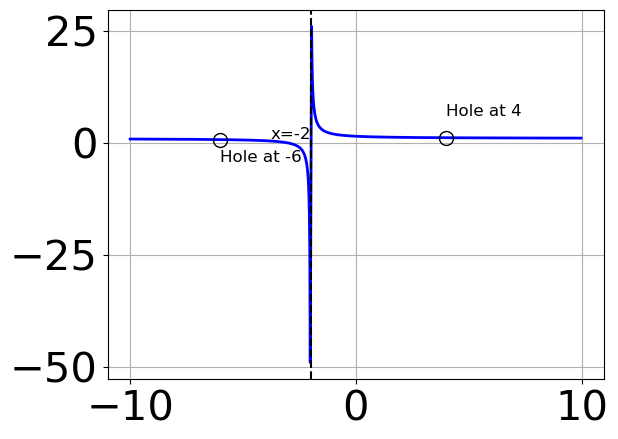
\includegraphics[width=0.5\textwidth]{../Figures/identifyGraphOfRationalFunctionCopyB.png}
\end{center}
\begin{enumerate}[label=\Alph*.]
\item \( f(x)=\frac{x^{3} +8.0 x^{2} -3.0 x -90.0}{x^{3} -4.0 x^{2} -20.0 x + 48.0} \)
\item \( f(x)=\frac{x^{3} -6.0 x^{2} -9.0 x + 54.0}{x^{3} +4.0 x^{2} -20.0 x -48.0} \)
\item \( f(x)=\frac{x^{3} +5.0 x^{2} -18.0 x -72.0}{x^{3} +4.0 x^{2} -20.0 x -48.0} \)
\item \( f(x)=\frac{x^{3} -5.0 x^{2} -18.0 x + 72.0}{x^{3} -4.0 x^{2} -20.0 x + 48.0} \)
\item \( \text{None of the above are possible equations for the graph.} \)

\end{enumerate} }
\litem{
Determine the vertical asymptotes and holes in the rational function below.\[ f(x) = \frac{9x^{3} -12 x^{2} -20 x + 16}{9x^{2} -21 x + 10} \]\begin{enumerate}[label=\Alph*.]
\item \( \text{Vertical Asymptote of } x = 1.0 \text{ and hole at } x = 0.667 \)
\item \( \text{Vertical Asymptotes of } x = 1.667 \text{ and } x = -1.333 \text{ with a hole at } x = 0.667 \)
\item \( \text{Vertical Asymptote of } x = 1.667 \text{ and hole at } x = 0.667 \)
\item \( \text{Holes at } x = 1.667 \text{ and } x = 0.667 \text{ with no vertical asymptotes.} \)
\item \( \text{Vertical Asymptotes of } x = 1.667 \text{ and } x = 0.667 \text{ with no holes.} \)

\end{enumerate} }
\litem{
Determine the horizontal and/or oblique asymptotes in the rational function below.\[ f(x) = \frac{12x^{3} +71 x^{2} +130 x + 75}{4x^{2} -11 x -20} \]\begin{enumerate}[label=\Alph*.]
\item \( \text{Horizontal Asymptote at } y = 4.0 \)
\item \( \text{Oblique Asymptote of } y = 3x + 26. \)
\item \( \text{Horizontal Asymptote of } y = 3.0 \text{ and Oblique Asymptote of } y = 3x + 26 \)
\item \( \text{Horizontal Asymptote of } y = 3.0  \)
\item \( \text{Horizontal Asymptote of } y = 4.0 \text{ and Oblique Asymptote of } y = 3x + 26 \)

\end{enumerate} }
\litem{
Determine the horizontal and/or oblique asymptotes in the rational function below.\[ f(x) = \frac{5x^{2} +24 x + 16}{20x^{3} +31 x^{2} -38 x -40} \]\begin{enumerate}[label=\Alph*.]
\item \( \text{Horizontal Asymptote at } y = -4.000 \)
\item \( \text{Horizontal Asymptote of } y = 0 \)
\item \( \text{Oblique Asymptote of } y = 4x -13. \)
\item \( \text{Horizontal Asymptote of } y = 0.250 \text{ and Oblique Asymptote of } y = 4x -13 \)
\item \( \text{Horizontal Asymptote of } y = 0.250  \)

\end{enumerate} }
\litem{
Determine the vertical asymptotes and holes in the rational function below.\[ f(x) = \frac{12x^{3} -5 x^{2} -17 x + 10}{12x^{2} -17 x + 6} \]\begin{enumerate}[label=\Alph*.]
\item \( \text{Vertical Asymptote of } x = 1.0 \text{ and hole at } x = 0.667 \)
\item \( \text{Vertical Asymptotes of } x = 0.75 \text{ and } x = 0.667 \text{ with no holes.} \)
\item \( \text{Vertical Asymptote of } x = 0.75 \text{ and hole at } x = 0.667 \)
\item \( \text{Vertical Asymptotes of } x = 0.75 \text{ and } x = -1.25 \text{ with a hole at } x = 0.667 \)
\item \( \text{Holes at } x = 0.75 \text{ and } x = 0.667 \text{ with no vertical asymptotes.} \)

\end{enumerate} }
\litem{
Determine the horizontal and/or oblique asymptotes in the rational function below.\[ f(x) = \frac{16x^{3} -16 x^{2} -9 x + 9}{4x^{2} -9 x -9} \]\begin{enumerate}[label=\Alph*.]
\item \( \text{Oblique Asymptote of } y = 4x + 5. \)
\item \( \text{Horizontal Asymptote of } y = 4.0  \)
\item \( \text{Horizontal Asymptote at } y = 3.0 \)
\item \( \text{Horizontal Asymptote of } y = 3.0 \text{ and Oblique Asymptote of } y = 4x + 5 \)
\item \( \text{Horizontal Asymptote of } y = 4.0 \text{ and Oblique Asymptote of } y = 4x + 5 \)

\end{enumerate} }
\litem{
Determine the horizontal and/or oblique asymptotes in the rational function below.\[ f(x) = \frac{8x^{3} +42 x^{2} +67 x + 30}{8x^{3} +50 x^{2} +85 x + 50} \]\begin{enumerate}[label=\Alph*.]
\item \( \text{Vertical Asymptote of } y = -2  \)
\item \( \text{Horizontal Asymptote of } y = 0  \)
\item \( \text{Vertical Asymptote of } y = -1.250  \)
\item \( \text{Horizontal Asymptote of } y = 1.000  \)
\item \( \text{None of the above} \)

\end{enumerate} }
\litem{
Which of the following functions \textit{could} be the graph below?
\begin{center}
    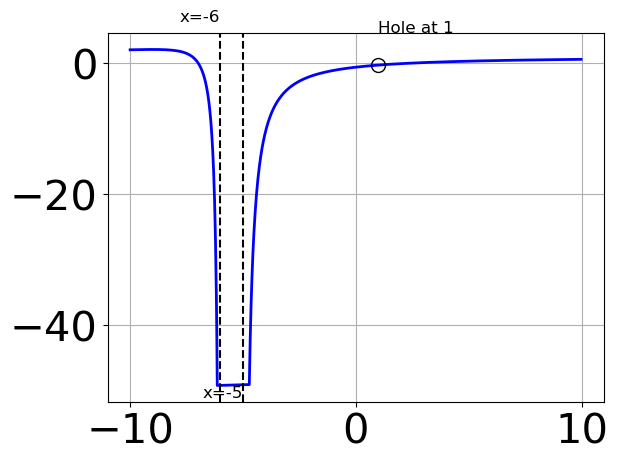
\includegraphics[width=0.5\textwidth]{../Figures/identifyGraphOfRationalFunctionB.png}
\end{center}
\begin{enumerate}[label=\Alph*.]
\item \( f(x)=\frac{x^{3} -3.0 x^{2} -25.0 x -21.0}{x^{3} -10.0 x^{2} +19.0 x + 30.0} \)
\item \( f(x)=\frac{x^{3} +2.0 x^{2} -29.0 x + 42.0}{x^{3} +10.0 x^{2} +19.0 x -30.0} \)
\item \( f(x)=\frac{x^{3} +3.0 x^{2} -25.0 x + 21.0}{x^{3} +10.0 x^{2} +19.0 x -30.0} \)
\item \( f(x)=\frac{x^{3} -7.0 x^{2} -9.0 x + 63.0}{x^{3} -10.0 x^{2} +19.0 x + 30.0} \)
\item \( \text{None of the above are possible equations for the graph.} \)

\end{enumerate} }
\end{enumerate}

\end{document}